% !TeX spellcheck = en_US
\addscenariosection{1}{Clash Scenario}{Arcane Artillery}{\images/precision.png}

\begin{multicols}{2}

\textbf{Author:} NeuroN

\textbf{Source:} \href{https://discord.com/channels/740870068178649108/1279029213839626313}{Archon Studios Discord}

\textit{The ancient ruins are filled with arcane magic and technology, we must take control of them before our enemies can.
Some pieces of arcane artillery are scattered aRound the ruins, they can help us kill the dragons resting in them.}

\subsection*{\MakeUppercase{Scenario Length}}
This Scenario is played over 12 Rounds.

\subsection*{\MakeUppercase{Player Setup}}
\textbf{Player Count:} 2-6 Player FFA or 2vs2, 2vs2vs2, 3vs3 Alliance

\textbf{Starting Resources:} 10 \svg{gold}, 6 \svg{building_materials}, 1 \svg{valuables}

\textbf{Starting Income:} 15 \svg{gold}, 2 \svg{building_materials}, 1 \svg{valuables}

\textbf{Starting Units:}
\begin{itemize}
  \item a Few of each \svgunit{bronze} Unit
\end{itemize}

\textbf{Town Buildings:} \svgunit{bronze} Dwelling

\textbf{Map Tile Pool:} Each player takes 1 random Far (II--III) Map Tile, it must contain a Settlement

\subsection*{\MakeUppercase{Map Setup}}
Take the following Map Tiles and arrange them as shown in the Scenario map layout:

\begin{itemize}
  \item If playing Alliance mode, alternate starting Tile placement such that allies do not start adjacent to each other.
\end{itemize}

\textbf{For a 2-player Scenario:}
\begin{itemize}
  \item 2 × Starting (I) Map Tile
  \item 4 × Near (IV--V) Map Tile that contains an Obelisk. If not enough are available, treat Witch Huts as Obelisks
  \item 1 × Center (VI--VII) Map Tile, which must contain the Dragon Utopia Field
\end{itemize}

\textbf{For a 3-6 player Scenario:}
\begin{itemize}
  \item P × Starting (I) Map Tile
  \item 6 × Near (IV--V) Map Tile that contains an Obelisk. If not enough are available, treat Witch Huts as Obelisks
  \item 1 × Center (VI--VII) Map Tile, which must contain the Dragon Utopia Field
\end{itemize}

\subsection*{\MakeUppercase{Victory Conditions}}
To win the Scenario, a Hero must Flag the Dragon Utopia Field.

\subsection*{\MakeUppercase{Defeat Conditions}}
At the end of the \nth{12} Round, if there is no winner, all players lose the Scenario.

\subsection*{\MakeUppercase{Timed Events}}

\textbf{\nth{6} Round:}
\begin{itemize}
  \item Remove all Black cubes from every Tile.
\end{itemize}

\subsection*{\MakeUppercase{Additional Rules}}

During this Scenario:

\begin{itemize}
  \item Heroes cannot enter starting Tiles other than their own.
  \item A Player may not use the Diplomacy card to skip Combat on the Dragon Utopia Field.
  \item Arcane Spikes are represented by cubes not used by any player's Faction.
  \item Obelisks may be Flagged. 
  \item Each Obelisk can only be Flagged by one Player at a time.
  \item When first Flagged, that Player gains one Arcane Spike.
  \item At the start of each Player's turn, that Player removes any unspent Arcane Spikes, then gains Arcane Spikes equal to the number of captured Obelisks they have.
\end{itemize}

\vspace{1em}

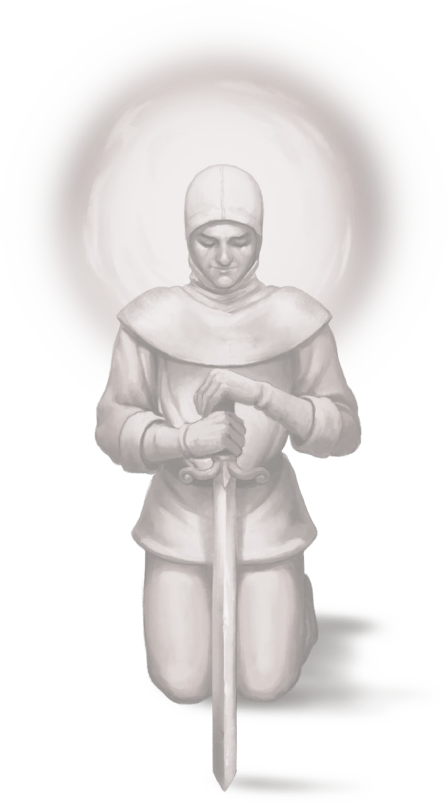
\includegraphics[width=\linewidth, keepaspectratio]{\art/prayer.png}

\vspace*{\fill}

\columnbreak

\textbf{Players can spend one Arcane Spike during combat to cast:}

\hommtable[]{15}{
  \begin{tabularx}{\linewidth}{X}
    \darkcell{\raisebox{-.2\height}{} \textbf{Arcane Artillery}}\\
    \lightcell[1.8]{\raisebox{-.25\height}{\svg{activation_white}} Deal 1 \svg{damage-table} to target Unit by placing an Arcane Spike on it.} \\ 
    \lightcell[3.8]{\raisebox{-.25\height}{\svg{ongoing_white}} A Unit with an Arcane Spike placed on it has its special ability negated \\ and receives +1 \svg{damage-table} from every source of \\ \svg{damage-table} and attacks for every Arcane Spike placed on them (even if they were to receive 0 damage)} \\
  \end{tabularx}
}

\textbf{Additionally:}

\begin{itemize}
  \item Arcane Artillery ignores Azure Dragon's Special Ability when cast during level VII combat.
  \item Arcane Artillery does not count toward your combat Round Spell limit.
  \item Arcane Artillery is considered to be a Spell of every school of magic of \svg{empower} 0
  \item Players can cast Srcane Srtillery during combat involving opponent's Heroes during the neutral unit's activation
  \item Each player can cast only one Arcane Artillery per combat round
  \item \textit{In alliance mode, allies can cast Arcane Artillery on allied Unit's activation}
\end{itemize}

\end{multicols}

\newpage

  \begin{minipage}{0.4\paperwidth}
    \centering
    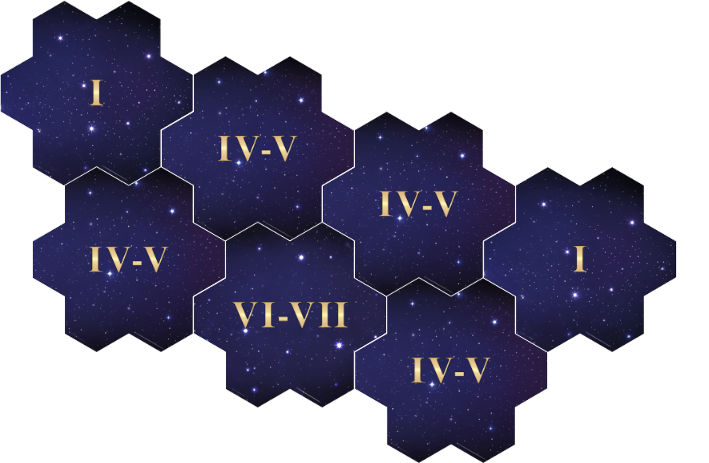
\includegraphics[width=0.36\paperwidth]{\maps/arcane_artillery_2p.png}
    \captionof{figure}{\textbf{2-PLAYER SCENARIO}}
  \end{minipage}
  \vspace{1em}
  \linebreak
  \begin{minipage}{0.4\paperwidth}
    \centering
    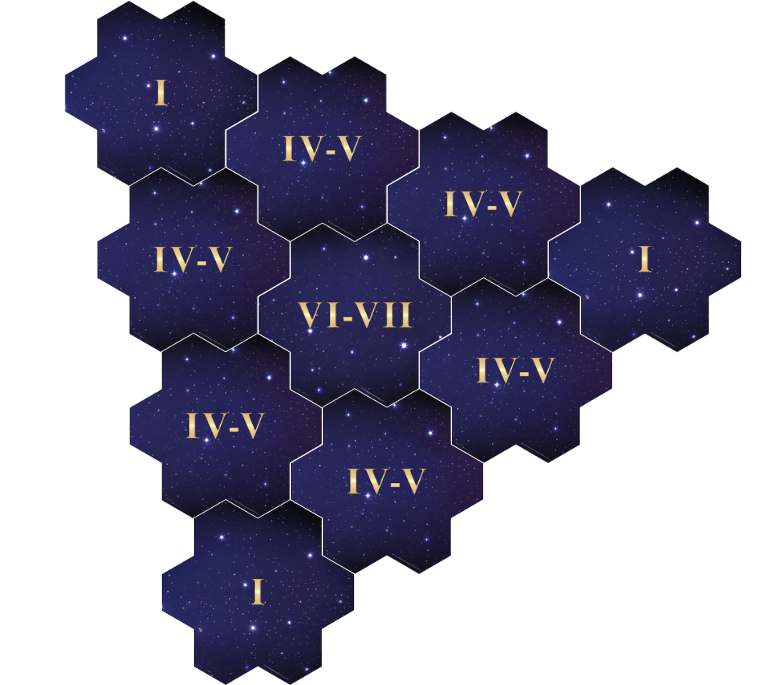
\includegraphics[width=0.38\paperwidth]{\maps/arcane_artillery_3p.png}
    \captionof{figure}{\textbf{3-PLAYER SCENARIO}}
  \end{minipage}
  \begin{minipage}{0.4\paperwidth}
    \centering
    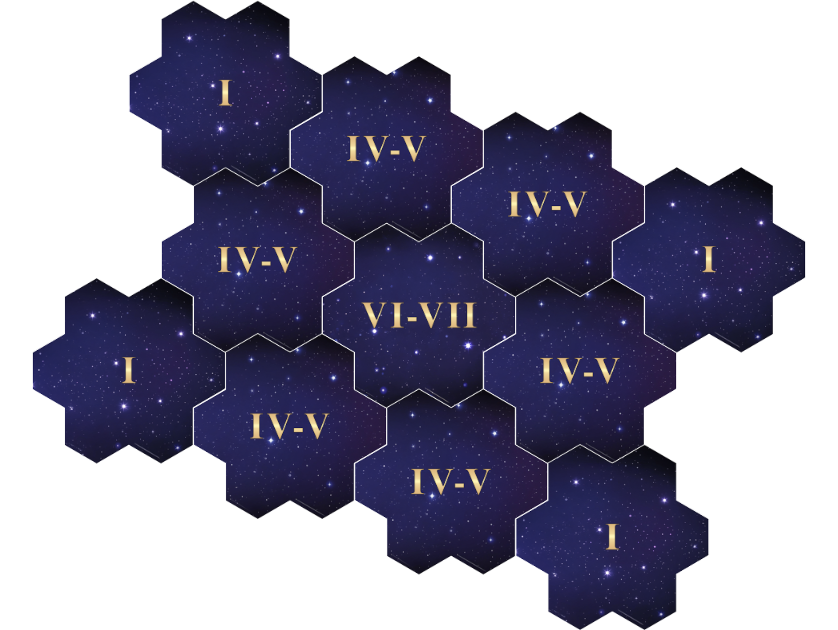
\includegraphics[width=0.38\paperwidth]{\maps/arcane_artillery_4p.png}
    \captionof{figure}{\textbf{4-PLAYER SCENARIO}}
  \end{minipage}
  \vspace{1em}
  \linebreak
  \begin{minipage}{0.4\paperwidth}
    \centering
    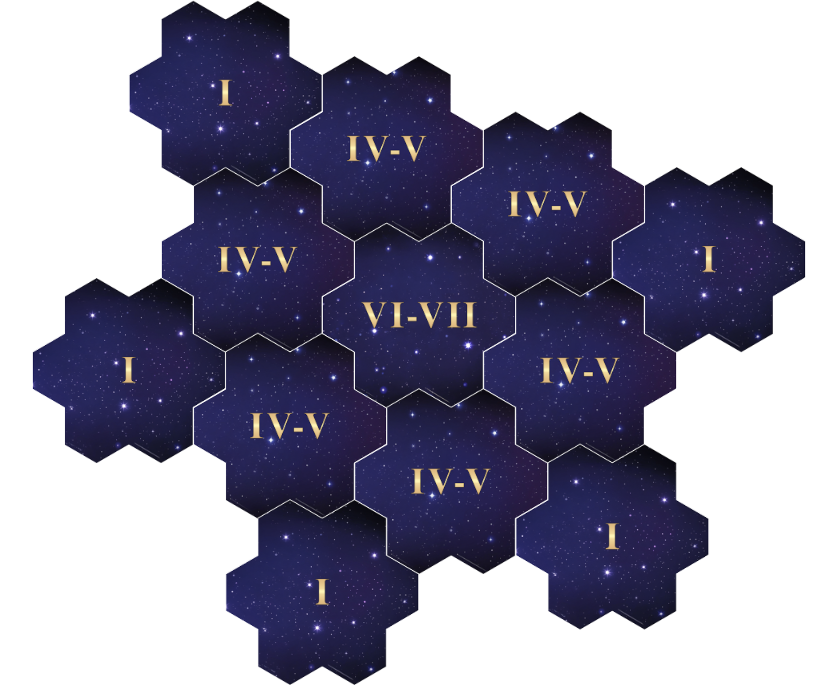
\includegraphics[width=0.38\paperwidth]{\maps/arcane_artillery_5p.png}
    \captionof{figure}{\textbf{5-PLAYER SCENARIO}}
  \end{minipage}
  \begin{minipage}{0.4\paperwidth}
    \centering
    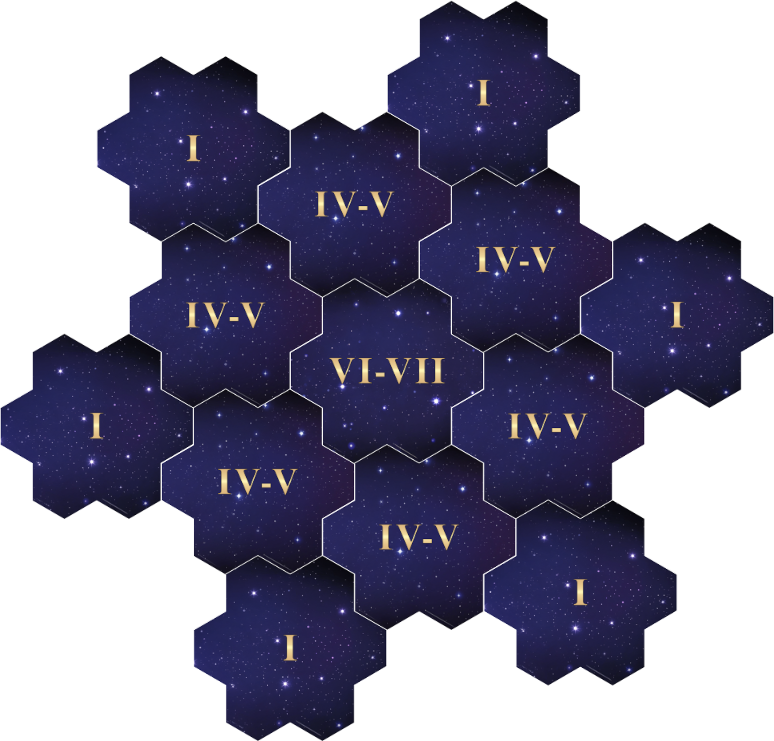
\includegraphics[width=0.38\paperwidth]{\maps/arcane_artillery_6p.png}
    \captionof{figure}{\textbf{6-PLAYER SCENARIO}}
  \end{minipage}
